\iffalse
\documentclass[journal,12pt,twocolumn]{IEEEtran}
\usepackage[none]{hyphenat}
\usepackage{graphicx}
\usepackage{listings}
\usepackage[english]{babel}
\usepackage{graphicx}
\usepackage{caption} 
\usepackage{amsmath}
\usepackage{hyperref}
\usepackage{booktabs}
\usepackage{array}
\let\vec\mathbf
\title{\textbf{\\Line Assignment}}
\author{Sinkona Chinthamalla - FWC22054}
\begin{document}
\maketitle

\section{Question}
\textbf{\textit{Class 11, Exercise 10.1, Q(1):}
\fi
Draw a quadrilateral in the Cartesian plane, whose vertices are 
(-4,5), (0,7), (5,-5), (-4,-2). Also, find its area.
\\
\solution See Fig. 
		\ref{fig:11/10/1/1}.
	\begin{figure}[!ht]
		\centering
 \includegraphics[width=\columnwidth]{chapters/11/10/1/1/figs/quadrilateral.png}
		\caption{}
		\label{fig:11/10/1/1}
  	\end{figure}
\iffalse
}

\begin{figure}[h!]
\centering
\includegraphics[scale=0.35]{quadrilateral.png}
\centering
\caption{Quadrilateral ABCD}
\end{figure}

\section{Construction}
\centering
\vspace{0.2cm}
{
\setlength\extrarowheight{2pt}
\begin{tabular}{|c|c|c|}
	\hline
	\textbf{Symbol}&\textbf{Value}&\textbf{Description}\\
	\hline
	A & $\begin{pmatrix}
     -4 \\
      5 
    \end{pmatrix}$ & Vertex A\\
	\hline
	B & $\begin{pmatrix}
     0 \\
     7 
    \end{pmatrix}$ & Vertex B\\
	\hline
	C & $\begin{pmatrix}
      5 \\
     -5 
    \end{pmatrix}$ & Vertex C\\
	\hline
	D & $\begin{pmatrix}
     -4 \\
     -2 
    \end{pmatrix}$ & Vertex D\\
	\hline
\end{tabular}
}

\section{Solution}
\raggedright 
We can divide the quadrilateral into two triangles, one with sides \textbf{AB}, \textbf{BC}, and \textbf{AC}, and the other with sides \textbf{AC}, \textbf{CD}, and \textbf{AD}.\\
\vspace{0.2cm}
\textbf{1. Finding area using Matrices} \\
\vspace{0.25cm}
Consider $ \triangle ABC, $
\vspace{0.2cm}
\begin{equation}
ar(\triangle \vec{ABC})= \frac{1}{2} \myvec{
                    \vec{x_1} & \vec{y_1} & 1\\
                    \vec{x_2} & \vec{y_2} & 1\\
                    \vec{x_3} & \vec{y_3} & 1
                   } 
\end{equation} 
\begin{center}
$ = \frac{1}{2} \myvec{
                    -4 & 5 & 1\\
                     0 & 7 & 1\\
                     5 & -5 & 1
                   } $ \\
                   \vspace{0.2cm}
\end{center}
\vspace{0.2cm}
\raggedright
\begin{equation}
ar(\triangle ABC)= 29 \quad sq.units 
\end{equation}  
\\( Since area cannot be negative )

\begin{figure}[h]
\centering
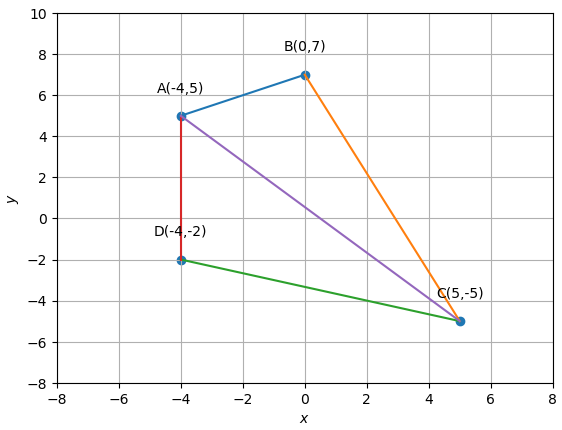
\includegraphics[scale=0.35]{diagnol.png}
\centering
\caption{Quadrilateral ABCD with diagonal AC}
\end{figure}

\vspace{0.3cm}
\noindent Now consider $ \triangle ADC, $
\begin{equation}
ar(\triangle \vec{ADC})= \frac{1}{2} \myvec{
                    \vec{x_1} & \vec{y_1} & 1\\
                    \vec{x_2} & \vec{y_2} & 1\\
                    \vec{x_3} & \vec{y_3} & 1
                   } 
\end{equation} 
\begin{center}
$ = \frac{1}{2} \myvec{
                    -4 &  5 & 1\\
                    -4 & -2 & 1\\
                     5 & -5 & 1
                   } $
\end{center}
\vspace{0.2cm}
\begin{equation}
ar(\triangle ADC)= 31.5 \quad sq.units 
\end{equation}

\boldmath
\vspace{0.2cm}
\textbf{Area of Quadrilateral ABCD} 
\begin{equation}
 = ar(\triangle ABC)+ar(\triangle ADC)
\end{equation}
\begin{center}
 = 60.5  sq.units
\end{center}

\newpage
\vspace{0.2cm} 
\textbf{2. Finding area using Cross product} \\
\vspace{0.25cm}
\fi
\begin{align}
	ar(\triangle ABC)&= \frac{1}{2}\norm{\brak{\vec{B}-\vec{A}} \times \brak{\vec{B}-\vec{C}}} 
	\\
	&= \frac{1}{2} \mydet{
                    4 & 2\\
                   -5 & 12
	   }
= 29 
\end{align}
Similarly,
\begin{align}
	ar(\triangle ADC)&= \frac{1}{2}\norm{\brak{\vec{D}-\vec{A}} \times \brak{\vec{D}-\vec{C}}}
	\\
	&= \frac{1}{2} \mydet{
                    0 & -7\\
                   -9 &  3
                   } 
= 31.5
\end{align}
Thus, 
\begin{align}
	ar(ABCD)
	&= ar(\triangle ABC)+ar(\triangle ADC) 
	= 60.5 
\end{align}

\iffalse
\vspace{1cm}
Get the python code from
\begin{table}[h]
\large
\centering
\begin{tabular}{|l|}
\hline
https://github.com/SinkonaChinthamalla/fwc/
\\blob/main/matrix/line/codes \\
\hline
\end{tabular}
\end{table}	
\end{document}
\fi
